\documentclass[12pt]{article}
\usepackage{placeins}
\usepackage{natbib}
%\VignetteIndexEntry{Hilbert Huang Transform Examples}
\usepackage{/usr/local/lib64/R/share/texmf/tex/latex/Sweave}
\begin{document}
\setkeys{Gin}{width=1\linewidth}
\title{Investigating some Interesting Signals with Hilbert and Fourier Spectrograms}
\author{Daniel Bowman}
\date{\today}
\maketitle
\tableofcontents


\section{Stacked Sinusoids I}

The Fourier method uses linear combinations of sinusoids as basis functions.
Therefore, it is reasonable to compare the performance of the HHT with the performance of the Fourier method
using a ``nice'' signal consisting of linear combinations of sinusoids.
This example shows the efficacy of the empirical mode decomposition (EMD) method and the equivalence of the HHT and Fourier spectrograms. 

The signal used for this example consists of four sinusoids: 

\begin{equation}
\label{eqn:stacked1}
x(t) =0.5\sin(\frac{\pi}{10} t) + \sin(2\pi t) + 0.5\sin(10\pi t) + 0.5\sin(40\pi t)
\end{equation}

The EMD of this signal produces 5 intrinsic mode functions (IMFs).
The first four IMFs correspond to the four sinusoids that comprise the signal (Fig. \ref{fig:stacked1imfs}).
The fifth IMF is a very low amplitude, long period signal probably corresponding to slight spline fitting errors or digitalization of the signal.
The ensemble Hilbert spectrogram of these IMFs show energy bands located at 0.05, 1, 5, and 20 Hz, respectively (Fig. \ref{fig:stacked1farhspec}), 
corresponding to the terms in Equation \ref{eqn:stacked1}.
The power of each frequency band corresponds to the amplitudes of each term in Equation \ref{eqn:stacked1}, where the 0.05, 5, and 20 Hz bands have
an amplitude of 0.5 and the 1 Hz band has an amplitude of 1.

The Fourier spectrogram resembles the Hilbert spectogram for the most part (Fig. \ref{fig:stacked1ft}).
The frequency resolution depends on the length of the time window, which in the case of this figure is less than the longest period.
Therefore, the spectrogram shows the first three components (1, 5, and 20 Hz) but not the fourth (0.05 Hz) component.
The amplitudes in the Fourier spectrogram do not bear as obvious a relationship with the terms of Equation \ref{eqn:stacked1} as does the Hilbert spectrogram.

In this example, the Hilbert and Fourier spectrograms were quite similar. 
The Hilbert spectrogram is slightly better because it does not require windowing and the spectral amplitudes bear a clearer relationship to the terms of the signal equation.
Of course, the sensible way to do Fourier analysis for a stationary signal such as this one is to simply display the periodogram - the spectrogram was shown merely to compare it to the Hilbert spectrogram.

\subsection{Code}

\textbf{Set up signal and perform EMD}
\begin{Schunk}
\begin{Sinput}
> library(hht)
> dt=0.01
> tt=seq_len(10000)*dt
> sig=0.5*sin(pi*tt/10)+sin(2*pi*tt)+0.5*sin(10*pi*tt)+0.5*sin(40*pi*tt)
> emd_config=list()
> emd_config$max_sift=200
> emd_config$max_imf=100
> emd_config$tol=5
> emd_config$stop_rule="type5"
> emd_config$boundary="wave"
> emd_config$sm="none"
> emd_config$spar=NA
> emd_config$weight=20
> emd_result=sig2imf(sig, dt, emd_config)
> emd_result=hhtransform(emd_result)
\end{Sinput}
\end{Schunk}

\textbf{Plot original signal and IMFs.}
\begin{Schunk}
\begin{Sinput}
> time_span=c(0,40)
> imf_list=1:4
> os=TRUE
> res=FALSE
> plot_imfs(emd_result, time_span, imf_list, os, res)
\end{Sinput}
\end{Schunk}

\textbf{Generate Hilbert spectrogram of the stacked sinusoidal signal.}

\begin{Schunk}
\begin{Sinput}
> max_freq=25
> freq_step=0.1
> hspec=hh_render(emd_result, max_freq, freq_step)
\end{Sinput}
\end{Schunk}

\begin{Schunk}
\begin{Sinput}
> time_span=c(0, -1)
> freq_span=c(0, 25)
> amp_span=c(0, 1)
> hhspec_image(hspec, time_span, freq_span, amp_span, cex=1)
\end{Sinput}
\end{Schunk}

\textbf{Generate Fourier spectrogram}

\begin{Schunk}
\begin{Sinput}
> ft=list()
> ft$xt=sig
> ft$dt=dt
> ft$nfft=2048
> ft$ns=1000
> ft$nov=998
> amp_span=c(100,200)
> ftspec_image(ft, time_span, freq_span, amp_span, cex=1)
\end{Sinput}
\end{Schunk}

\FloatBarrier

\subsection{Figures}

\begin{figure}[h]
\begin{center}
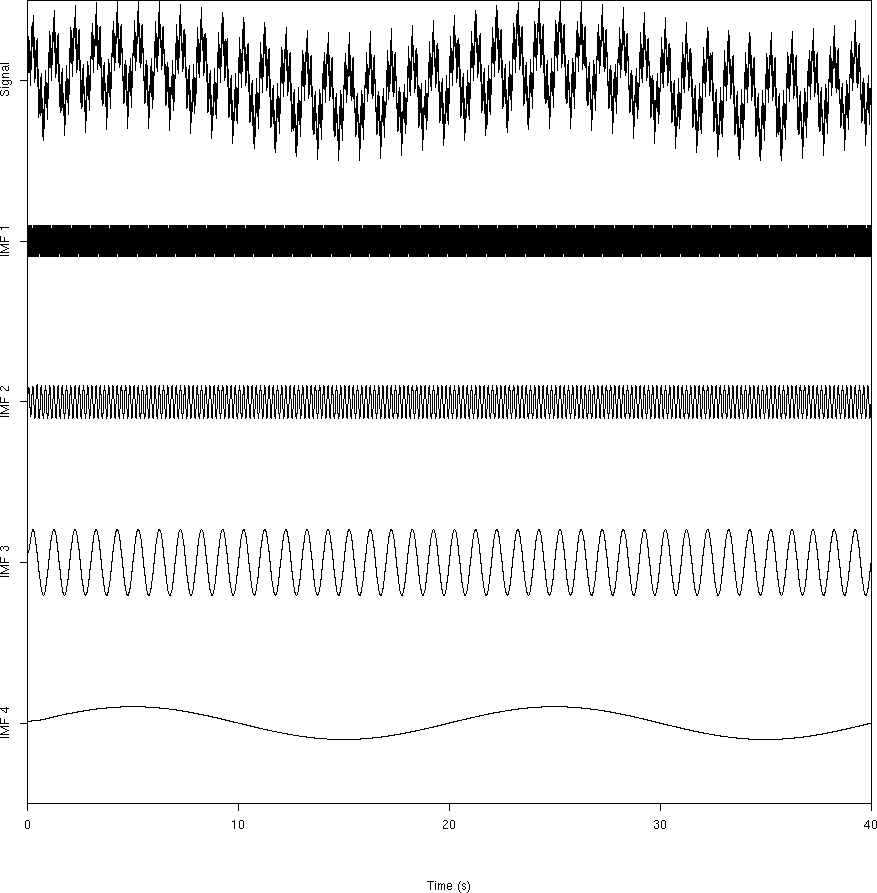
\includegraphics[width=1\textwidth]{stacked1imfs.png}
\end{center}
\caption{Empirical mode decomposition of stacked sinusoidal signal.}
\label{fig:stacked1imfs}
\end{figure}

\begin{figure}[h]
\begin{center}
%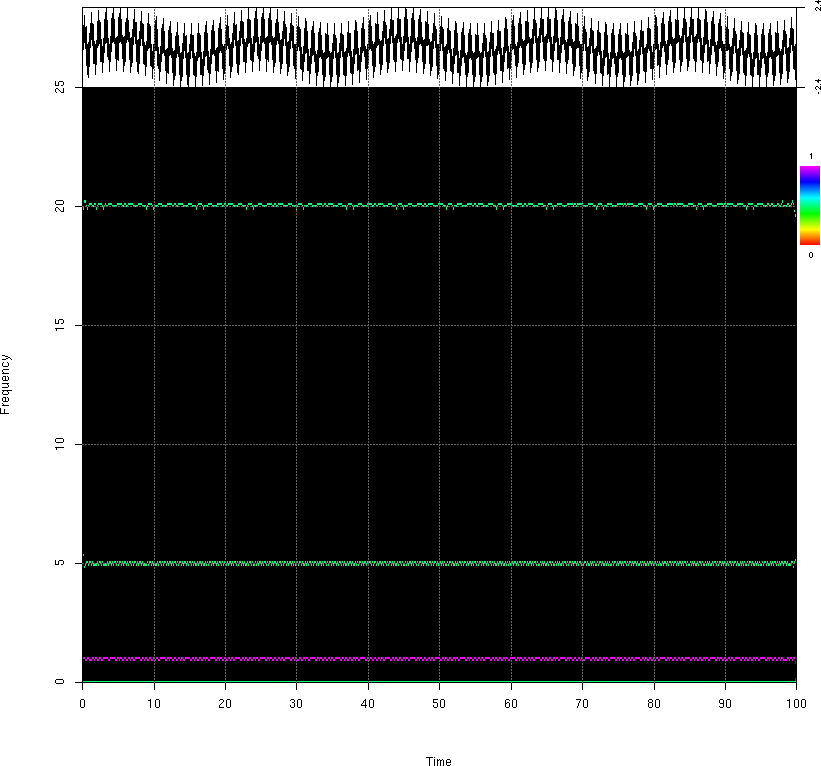
\includegraphics{stacked1farhspec.png}
\end{center}
\caption{Hilbert spectrogram of stacked sinusoids.  All four components are present in the spectrogram (the lowest frequency is a faint green line at the very bottom).}
\label{fig:stacked1farhspec}
\end{figure}

\begin{figure}[h]
\begin{center}
%\includegraphics{"stacked1ft.png"}
\end{center}
\caption{Fourier spectrum of stacked sinusoids.}
\label{fig:stacked1ft}
\end{figure}

\FloatBarrier

\section{Stacked Sinusoids II}

While the EMD method works well when each term produces extrema, it runs into serious trouble when linear combinations do not produce distinct riding and carrier waves.
In this case, the Hilbert spectrogram will produce a very different result than the Fourier spectrogram.
This problem can be illustrated by using the following signal:

\begin{equation}
\label{eqn:stacked2}
x(t) = \sin(2 \pi t) + 0.25\sin(4 \pi t)
\end{equation}

Since the riding wave does not produce independent extrema, the EMD cannot separate the two terms of the equation.
This means that the EMD produces only one IMF.
The IMF is a distorted sine wave consisting of the sum of the first and second terms of the equation (Fig. \ref{fig:stacked2imf}).
The Hilbert spectrogram displays this as a frequency modulation (Fig. \ref{fig:stacked2ht}).
However, the Fourier spectrogram shows two distinct bands, one at 1 Hz and the other at 2 Hz (Fig. \ref{fig:stacked2ft}).
Thus the Fourier spectrogram reflects the terms of Equation \ref{eqn:stacked2}, and the Hilbert spectrogram does not.
This and other shortcomings of the EMD method are discussed extensively in D\"{a}tig and Schlurmann (2004).

\subsection{Code}

\textbf{Set up signal, perform EMD, and plot IMFs}
\begin{Schunk}
\begin{Sinput}
> library(hht)
> dt=0.05
> tt=seq_len(10000)*dt
> sig=sin(2*pi*tt)+0.25*sin(4*pi*tt)
> emd_config=list()
> emd_config$max_sift=200
> emd_config$max_imf=100
> emd_config$tol=5
> emd_config$stop_rule="type5"
> emd_config$boundary="wave"
> emd_config$sm="none"
> emd_config$spar=NA
> emd_config$weight=20
> emd_result=sig2imf(sig, dt, emd_config)
> time_span=c(20, 30)
> imf_list=c(1)
> os=TRUE
> res=FALSE
> fit_line=TRUE
> plot_imfs(emd_result, time_span, imf_list, os, res, fit_line)
\end{Sinput}
\end{Schunk}


\textbf{Hilbert spectrogram}
\begin{Schunk}
\begin{Sinput}
> emd_result=hhtransform(emd_result)
> max_freq=4
> freq_step=0.1
> imf_list=c(1)
> hspec=hh_render(emd_result, max_freq, freq_step, imf_list)
\end{Sinput}
\end{Schunk}

\begin{Schunk}
\begin{Sinput}
> time_span=c(20, 30)
> freq_span=c(0, 3)
> amp_span=c(0, -1)
> hhspec_image(hspec, time_span, freq_span, amp_span, cex=1)
\end{Sinput}
\end{Schunk}

\textbf{Fourier spectrogram}
\begin{Schunk}
\begin{Sinput}
> ft=list()
> ft$xt=sig
> ft$dt=dt
> ft$nfft=4096
> ft$ns=2000
> ft$nov=1998
> time_span=c(0, -1)
> freq_span=c(0, 3)
> amp_span=c(90, 200)
> ftspec_image(ft, time_span, freq_span, amp_span, cex=1)
\end{Sinput}
\end{Schunk}

\subsection{Figures}

\FloatBarrier

\begin{figure}[h]
\begin{center}
%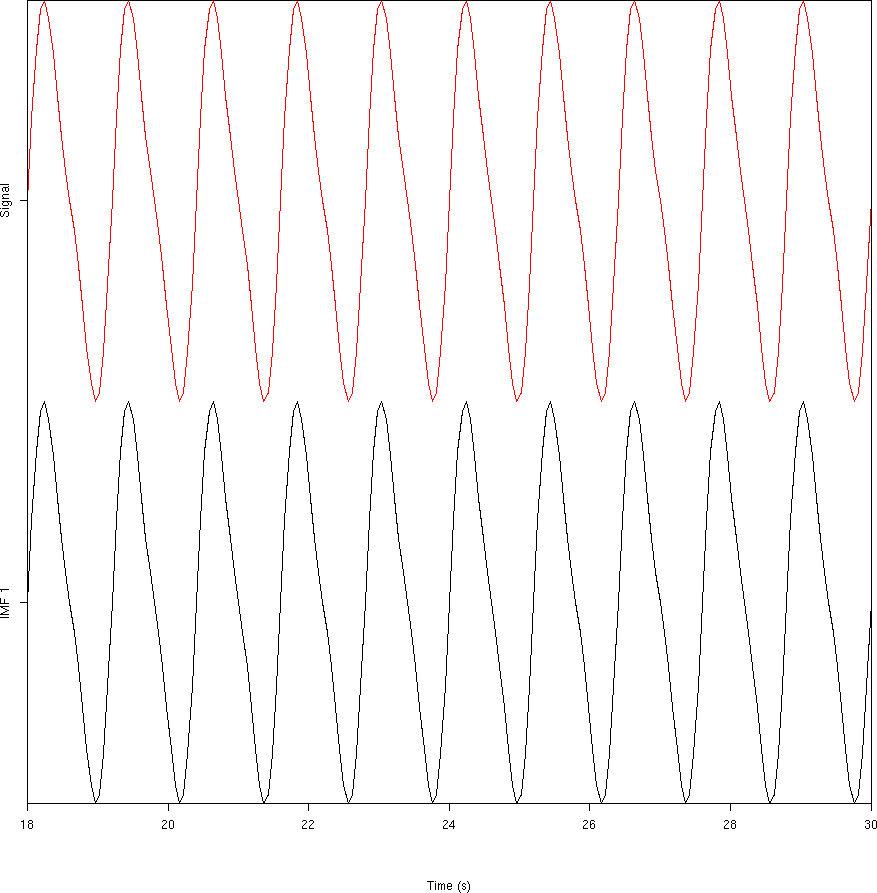
\includegraphics{stacked2imf.png}
\end{center}
\caption{EMD of the stacked sinusoidal signal in Equation \ref{eqn:stacked2}
The red line on the ``Signal'' portion of the plot denotes the contribution of IMF 1 to the total signal (black line)
Evidently IMF 1 contains almost all the variability of the signal.}
\label{fig:stacked2imf}
\end{figure}

\begin{figure}[h]
\begin{center}
%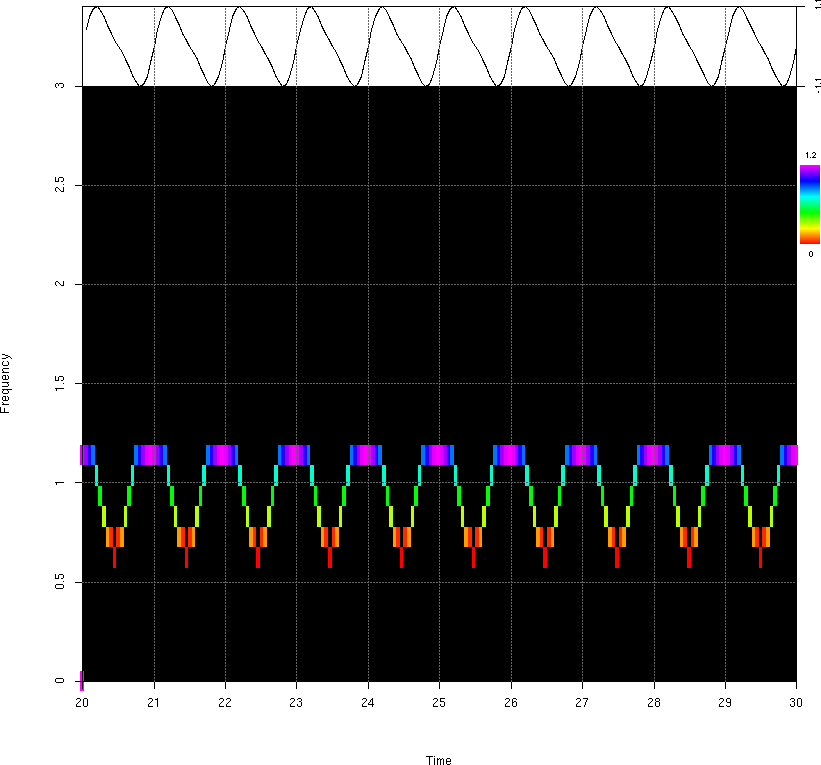
\includegraphics{stacked2ht.png}
\end{center}
\caption{Hilbert spectrogram of signal from Equation \ref{eqn:stacked2}.}
\label{fig:stacked2ht}
\end{figure}

\begin{figure}[h]
\begin{center}
%\includegraphics{fig:stacked2ft}
\end{center}
\caption{Fourier spectrogram of signal from Equation \ref{eqn:stacked2}.}
\label{fig:stacked2ft}
\end{figure}

\FloatBarrier

\section{Nonlinear and Nonstationary Signal}

While the Fourier spectrogram is essentially equivalent to or superior to the Hilbert spectrogram for linear and stationary signals,
the true power of the HHT emerges when the signals are neither linear nor stationary.
Here, we investigate a frequency modulated wave with a normal taper combined with high and low frequency sinusoidal waves:

\begin{equation}
\label{eqn:nonlinsta}
x (t) = \sin(2\pi t+0.5\sin(\pi t))e^{\frac{-(t-50)^{2})}{200}} + \sin(\frac{\pi}{10} t)
\end{equation}

The EMD successfully separates the components of the signal (Fig. \ref{fig:nonlinstaimfs}).
The Hilbert spectrogram describes the signal as a frequency modulated trace centered around 1 Hz and a 
sinusoidal trace centered at 0.1 Hz (Fig. \ref{fig:nonlinstaht}).
However, the Fourier spectrogram shows several harmonics that are not implied by Equation \ref{eqn:nonlinsta} (Fig. \ref{fig:nonlinstaft}).
Additional aliasing is present at lower frequencies, perhaps because the window is not quite long enough to capture the 0.1 Hz signal.
The nonphysical harmonics in the Fourier spectrogram are a consequence of representing a nonlinear signal as a linear combination of sinusoids.
Note the spline fitting errors at the beginning and ending of the IMF set (Fig. \ref{fig:nonlinstaimfs}).
This issue is addressed in the vignette ``Improving the Performance of the HHT using Ensemble Empirical Mode Decomposition.''

\subsection{Code}

\textbf{Set up signal, perform EMD and plot IMFs}
\begin{Schunk}
\begin{Sinput}
> library(hht)
> dt=0.01
> tt=seq_len(10000)*dt
> sig=sin(2*pi*tt+0.5*sin(pi*tt))*exp(-(tt-50)^2/100)+sin(pi*tt/10)
> emd_config=list()
> emd_config$max_sift=200
> emd_config$max_imf=100
> emd_config$tol=5
> emd_config$stop_rule="type5"
> emd_config$boundary="wave"
> emd_config$sm="none"
> emd_config$spar=NA
> emd_config$weight=20
> emd_result=sig2imf(sig, dt, emd_config)
> time_span=c(0, -1)
> imf_list=c(1:2)
> os=TRUE
> res=TRUE
> plot_imfs(emd_result, time_span, imf_list, os, res)
\end{Sinput}
\end{Schunk}

\textbf{Hilbert spectrogram}

\begin{Schunk}
\begin{Sinput}
> emd_result=hhtransform(emd_result)
> max_freq=5
> freq_step=0.05
> hspec=hh_render(emd_result, max_freq, freq_step)
\end{Sinput}
\begin{Soutput}
[1] "Rendering spectrogram..."
[1] "10  percent complete..."
[1] "20  percent complete..."
[1] "30  percent complete..."
[1] "40  percent complete..."
[1] "50  percent complete..."
[1] "60  percent complete..."
[1] "70  percent complete..."
[1] "80  percent complete..."
[1] "90  percent complete..."
\end{Soutput}
\end{Schunk}

\begin{Schunk}
\begin{Sinput}
> time_span=c(0, 100)
> freq_span=c(0, 2.5)
> amp_span=c(0, 1)
> hhspec_image(hspec, time_span, freq_span, amp_span, cex=1)
\end{Sinput}
\end{Schunk}

\textbf{Fourier spectrogram}
\begin{Schunk}
\begin{Sinput}
> ft=list()
> ft$xt=sig
> ft$dt=dt
> ft$nfft=4096
> ft$ns=2000
> ft$nov=1998
> amp_span=c(100,200)
> ftspec_image(ft, time_span, freq_span, amp_span, cex=1)
\end{Sinput}
\begin{Soutput}
evolfft kcol= 4001 krow= 2048 Ns 2000 Nov 1998
\end{Soutput}
\end{Schunk}

\FloatBarrier

\subsection{Figures}

\begin{figure}[h]
\begin{center}
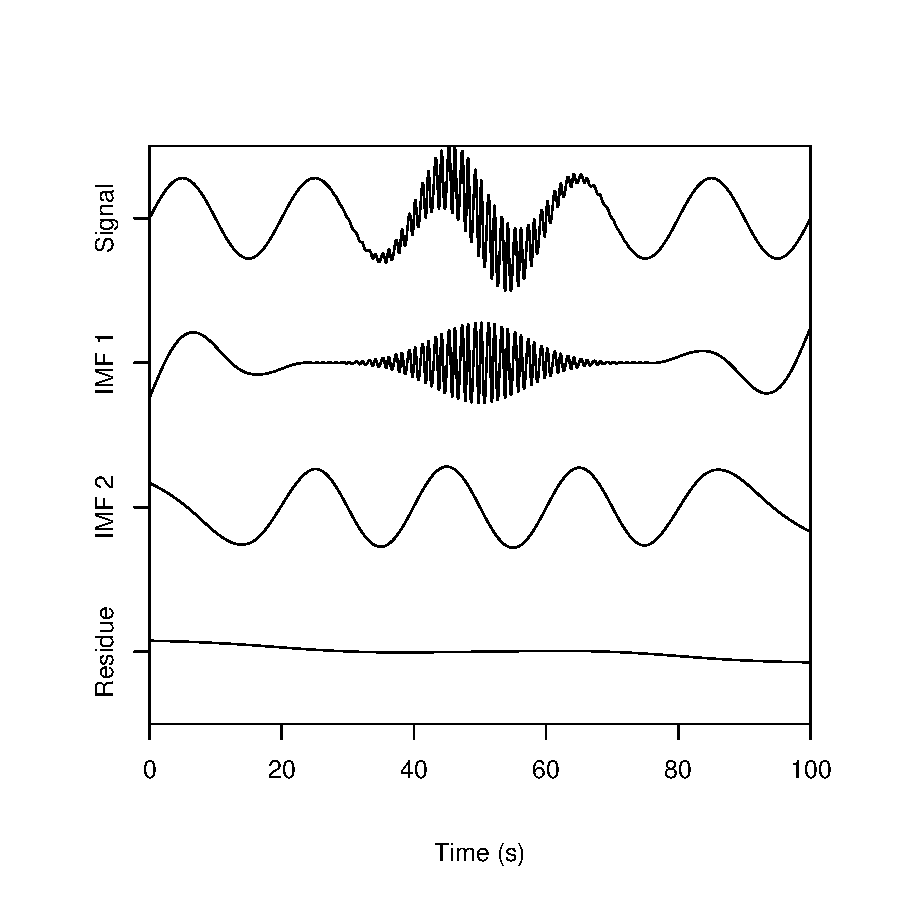
\includegraphics{interesting_signals-nonlinstaimfs}
\end{center}
\caption{EMD of signal in Equation \ref{eqn:nonlinsta}.
The distortions at the beginning and end of IMFs 2 and 3 are due to spline fitting errors.}
\label{fig:nonlinstaimfs}
\end{figure}

\begin{figure}[h]
\begin{center}
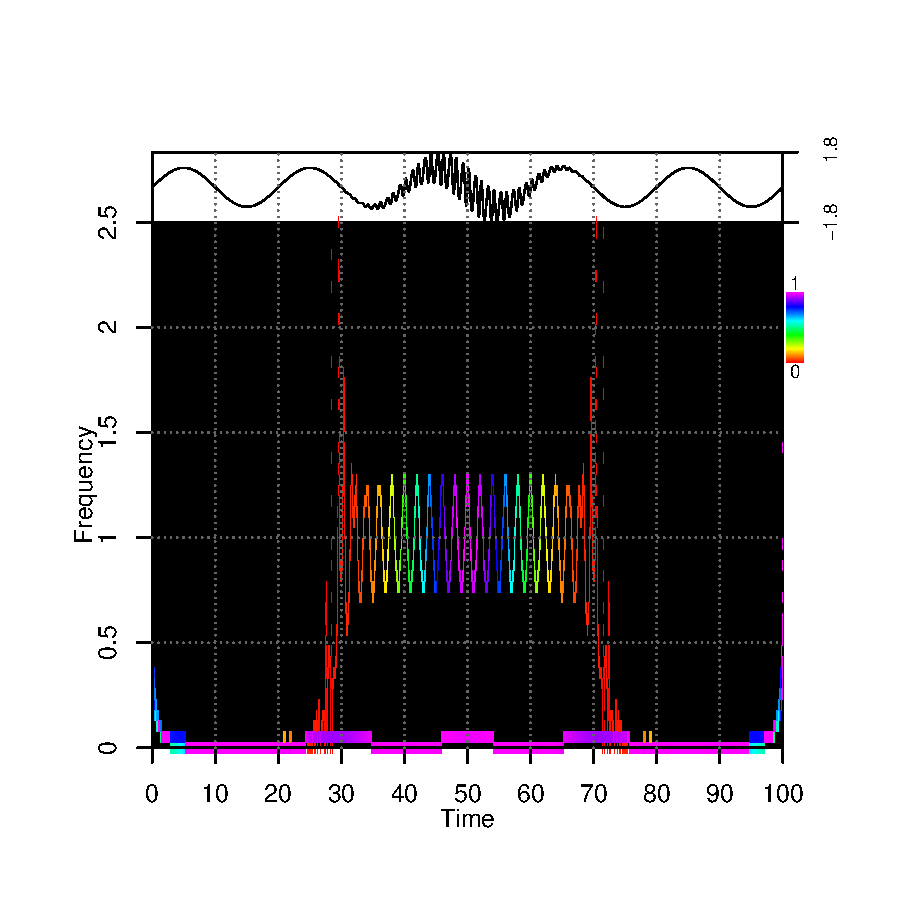
\includegraphics{interesting_signals-nonlinstaht}
\end{center}
\caption{Hilbert transform of signal in Equation \ref{eqn:nonlinsta}.}
\label{fig:nonlinstaht}
\end{figure}

\begin{figure}[h]
\begin{center}
\begin{Schunk}
\begin{Soutput}
evolfft kcol= 4001 krow= 2048 Ns 2000 Nov 1998
\end{Soutput}
\end{Schunk}
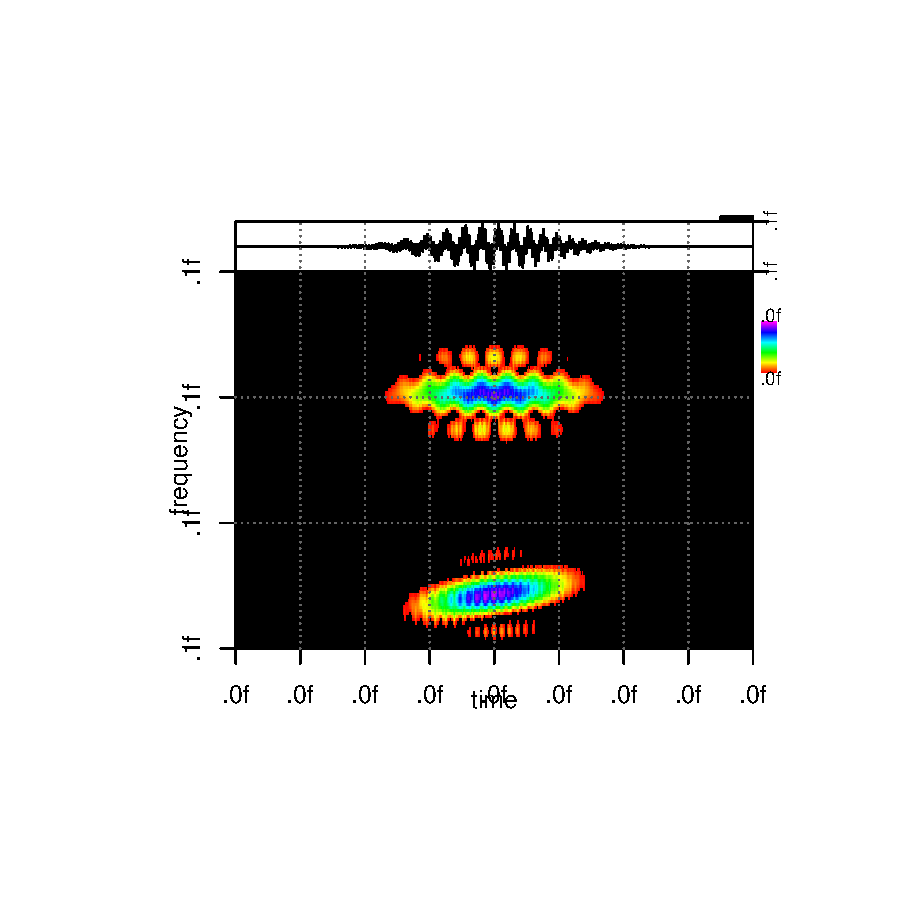
\includegraphics{interesting_signals-nonlinstaft}
\end{center}
\caption{Fourier transform of signal in Equation \ref{eqn:nonlinsta}.}
\label{fig:nonlinstaft}
\end{figure}

\end{document}
